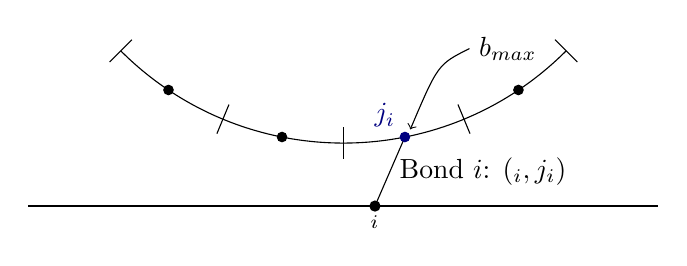
\begin{tikzpicture}
  [scale=4,
  midpoints/.style=blue!50!black,
  intervals/.style=red!50!black]
  \draw (225:1) arc [start angle=225, end angle=315, radius=1];
  \foreach \th in {-2,...,2}
  \draw (270 + 22.5*\th:.95) -- (270 + 22.5*\th:1.05);

  \draw[semithick] (-1, -1.2) -- (1, -1.2);
  \draw (281.25:1) -- node[right] {Bond $i$: $(\wallDist_i, j_i)$}
  (.1, -1.2);
  \filldraw[semithick] (.1, -1.2) node[below] {$\wallDist_i$} circle
  [radius=.015];
  
  \foreach \th in {236.25,258.75,303.75}
  \filldraw (\th:1) circle [radius=.015];
  
  \filldraw[midpoints] (281.25:1) node [above left] {$\binMidpoint{j_i}$}
  circle [radius=.015];

  \draw[->] (.4,-.7) node [right] {$b_\tn{max}$}
  .. controls (.3, -.75) .. (282.5:.98);
\end{tikzpicture}
